\documentclass{article}
\usepackage[a4paper, total={6in, 8in}]{geometry}

\usepackage{hyperref}
\usepackage{xcolor}
\usepackage{mathtools, nccmath}
\usepackage{algorithm}
\usepackage[noend]{algpseudocode}
\usepackage{graphicx}
\usepackage{listings}
\lstset{basicstyle=\ttfamily,
  showstringspaces=false,
  commentstyle=\color{red},
  keywordstyle=\color{blue}
}
\title{CFD Lab Group E Project Documentation}
\date{July 2021}
\author{
  Yunus Can Cakir\\
  \text{Technical University of Munich}
  \and
  Markus Mühlhäußer\\
  \text{Technical University of Munich}
  \and
   Sheng Chia-Yu\\
  \text{Technical University of Munich}
}
\begin{document}
\maketitle

\section{Introduction}
In this CFD project, our main goal was to implement and investigate different turbulent models. Aside from this, we wanted to explore different solvers, parallelization of our code on the GPU with different APIs, preconditioning, adaptive grid refinement and more. Our CFD solver comprises of 3 types of simulations: a CPU, a Vulkan and a CUDA simulation. It also supports MPI on the CPU path. During the course of our project we have implemented K-epsilon, K-omega and K-omega SST turbulent models.

\section{Code}
Our code diverges from the given skeleton in the sense that we have a single Solver class and depending on the simulation type we have CPUSolver, VulkanSolver or CudaSolver classes. In the Utilities.hpp file, you can change the precision between double and float under the "Real" type. Inside the Simulation.cpp file, the solver loop runs. The solver loop is divided into 3 sub methods that is implemented by each subclass. These are namely, 
\begin{lstlisting}[language=C++,frame=single]
void initialize()
\end{lstlisting}
This method handles all the initialization specific to chosen path. In Vulkan, this method handles preconditioner calculation, buffer allocation, descriptor binding etc. In CUDA, similarly this method handles preconditioner calculation and buffer allocation.
\begin{lstlisting}[language=C++,frame=single]
void solve_pre_pressure(Real &dt)
\end{lstlisting}
That handles the computations up to the pressure solving step. These include dt calculation, F and G calculation, setting up boundary values and other GPU or CPU specific tasks.
\begin{lstlisting}[language=C++,frame=single]
void solve_pressure(Real &res, uint32_t &it)
\end{lstlisting}
This method handles the pressure solving step. Depending on the configuration, either an SOR solver or a PCG solver is employed on the GPU or CPU.
\begin{lstlisting}[language=C++,frame=single]
void solve_post_pressure()
\end{lstlisting}
This method handles velocity calculation, turbulent viscosity, k/$\epsilon$ or $\omega$ calculation and copying the field values to the CPU for VTK output, if the GPU path is selected.

\subsection{Running the code}
The code has been tested on both Linux and Windows. For Linux you can build the code via CMake.
\begin{lstlisting}[language=bash,frame=single]
mkdir build
cd build
cmake ..
make
\end{lstlisting}
Make sure you enable CUDA or Vulkan support from the CMake settings.
\begin{itemize}
    \item Vulkan : cmake .. -DUSE\_VULKAN=ON
    \item CUDA : cmake .. -DUSE\_CUDA=ON
\end{itemize}
Make sure you delete you CMake cache if you change these settings midway through the build. \newline
Also note that the Vulkan code is only tested and designed on a RTX 3060 GPU, therefore there may be problems on lower-end hardware.
\subsection{Scene configuration}
In addition to the usual options from the previous exercises, we have other options.
\begin{itemize}
    \item model
    \begin{itemize}
        \item 0 $\rightarrow$ Turbulence off(default)
        \item 1 $\rightarrow$  K-epsilon model
        \item 2 $\rightarrow$  K-omega model
        \item 3 $\rightarrow$  K-omega SST model
    \end{itemize}
    \item solver
    \begin{itemize}
        \item 0 $\rightarrow$ SOR(default)
        \item 1 $\rightarrow$ PCG
    \end{itemize}
    \item simulation
    \begin{itemize}
        \item 0 $\rightarrow$ CPU(default)
        \item 1 $\rightarrow$ Cuda
        \item 2 $\rightarrow$ Vulkan
    \end{itemize}
    \item preconditioner
    \begin{itemize}
        \item -1 $\rightarrow$ off(default)
        \item 0 $\rightarrow$ AINV
        \item 1 $\rightarrow$ SSOR
        \item 2 $\rightarrow$ Jacobi preconditioner
    \end{itemize}
    \item refine
    \begin{itemize}
        \item Number (Grid has the refinement level $2^N$
    \end{itemize}
\end{itemize}

Note that following combinations are not supported:
\begin{itemize}
    \item PCG - MPI
    \item Cuda - MPI
    \item Vulkan - MPI
\end{itemize}


\section{Turbulent Models}
In our code we are using RANS-based turbulence modelds. Specifically we are using eddy viscosity models that models the turbulence via a turbulent viscosity term. 

\subsection{K-epsilon Model}
In this model, we model the turbulent viscosity as
\begin{equation}
\mu_{t}=\rho C_{\mu} \frac{k^{2}}{\epsilon}
\end{equation}
Where k is the kinetic energy and $\epsilon$ is the turbulent dissipation rate. \newline
We calculate these quantities via the equations:
\begin{equation}
\frac{\partial(\rho k)}{\partial t}+\frac{\partial\left(\rho k u_{i}\right)}{\partial x_{i}}=\frac{\partial}{\partial x_{j}}\left[\frac{\mu_{t}}{\sigma_{k}} \frac{\partial k}{\partial x_{j}}\right]+2 \mu_{t} E_{i j} E_{i j}-\rho \varepsilon
\end{equation}
\begin{equation}
\frac{\partial(\rho \varepsilon)}{\partial t}+\frac{\partial\left(\rho \varepsilon u_{i}\right)}{\partial x_{i}}=\frac{\partial}{\partial x_{j}}\left[\frac{\mu_{t}}{\sigma_{\varepsilon}} \frac{\partial \varepsilon}{\partial x_{j}}\right]+C_{1 \varepsilon} \frac{\varepsilon}{k} 2 \mu_{t} E_{i j} E_{i j}-C_{2 \varepsilon} \rho \frac{\varepsilon^{2}}{k}
\end{equation}

Although the K-epsilon model is fairly accurate away from the wall, it is problematic near the wall due to high shear stress, which results in higher $\mu$ along the walls.

\subsection{K-omega model}
Just like the K-epsilon model, the K-omega model is also a two equation model. Here, we reformulate the $\omega$ such that:
\begin{equation}
\omega=\frac{\epsilon}{C_{\mu} k} , C_{\mu} = 0.09
\end{equation}

Then we transport the quantities K and $\omega$ as usual.

Compared to K-epsilon model, the K-omega model has much better behaviour near walls, however one still wants the accuracy the K-epsilon model shows away from the walls. Which brings us to another widely used turbulence model.

\subsection{K-omega SST model}

In this model, we "blend" between K-omega and K-epsilon via a constant and limit the turbulent viscosity in the process. In the process, the only difference with the K-omega model is the limitation of the viscosity and the extra term in the $\omega$ transport. Namely,
\begin{equation}
\nu_{T}=\frac{a_{1} k}{\max \left(a_{1} \omega, S F_{2}\right)}
\end{equation}

\begin{equation}
\frac{\partial \omega}{\partial t}+U_{j} \frac{\partial \omega}{\partial x_{j}}=\alpha S^{2}-\beta \omega^{2}+\frac{\partial}{\partial x_{j}}\left[\left(\nu+\sigma_{\omega} \nu_{T}\right) \frac{\partial \omega}{\partial x_{j}}\right]+2\left(1-F_{1}\right) \sigma_{\omega 2} \frac{1}{\omega} \frac{\partial k}{\partial x_{i}} \frac{\partial \omega}{\partial x_{i}}
\end{equation}

Via constants $F_1$ and $F_2$. These are empirically derived constants fitted to a tanh function.

In our observations, we found that SST model is in between the K-epsilon and K-omega model, as suggested by the literature.

\begin{figure}
\centering
  \centering
  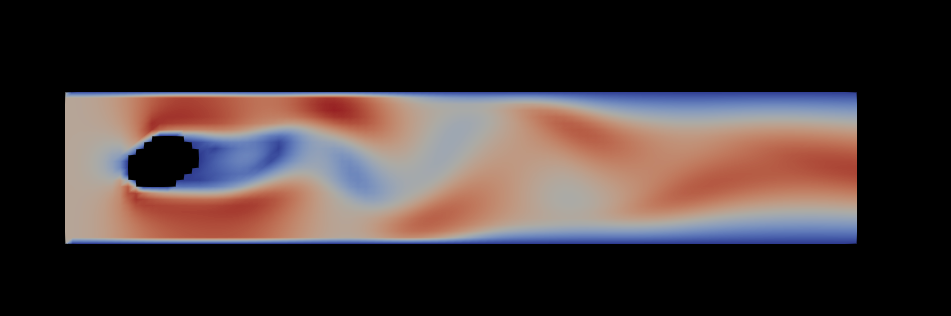
\includegraphics[width=.6\linewidth]{komega.png}
  \caption{K-omega model on Karman Vortex Street}
  \label{fig:sub1}
  \centering
  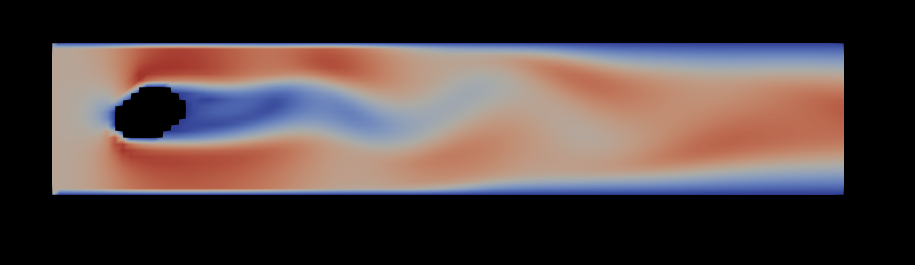
\includegraphics[width=.6\linewidth]{sst.png}
  \caption{K-omega SST model on Karman Vortex Street}
  \label{fig:sub2}
\label{fig:test}
\end{figure}

\section{Pressure Solvers and Preconditioners}
Aside from the usual SOR solver, we have added a PCG solver for the CPU, Vulkan and the CUDA path. For reference in the CPU path, we've used a modified version of Robert Bridson's PCG code which also provides a Modified Incomplete Cholesky preconditioner. In the GPU paths, we've implemented our own PCG solver and experimented with different preconditioners. For the preconditioners in the GPU branches, we wanted SPAI preconditioners for fast evaluation on the GPU, otherwise we'd have to solve 2 triangular systems which is a costly operation.

\subsection{Jacobi Preconditioner}
This is the simplest type of preconditioner. Since in our case the Laplacian matrix has non-zero diagonals, we simply use $P_{ij} = \frac{1}{D_{ij}}$ where D is the diagonal part of the pressure matrix.

\subsection{SSOR Preconditioner}

This preconditioner \cite{helfenstein} is defined by 
\begin{equation}
M=K K^{T}
\end{equation}
where 
\begin{equation}
K=\frac{1}{\sqrt{2-\omega}}(\bar{D}+L) \bar{D}^{-1 / 2}
\end{equation}
in which $0 <  \omega < 2$ and $\bar{D} = \frac{1}{\omega}D$
In the code, we precompute this matrix from the pressure matrix, then in the CG algorithm, the only extra cost is a sparse matrix vector multiplication.

\subsection{Approximate Inverse Preconditioner Variant}
This preconditioner \cite{labutin} approximates the inverse by first choosing an initial preconditioner, in which case we've chosen a Jacobi preconditioner, then approximating
the inverse via Neumann series. Assuming we have $D_0$ as an initial approximation of $A^{-1}$ and a condition 

\begin{equation}
\left\|R_{0}\right\| \leq k<1, \quad R_{0}=I-A D_{0}
\end{equation}
Then,
\begin{equation}
\begin{aligned}
A^{-1} &=\left(D_{0} D_{0}^{-1}\right) A^{-1}=D_{0}\left(D_{0}^{-1} A^{-1}\right) \\
&=D_{0}\left(A D_{0}\right)^{-1}=D_{0}\left(I-R_{0}\right)^{-1} \\
&=D_{0}\left(I+R_{0}+R_{0}^{2}+R_{0}^{3}+\ldots\right)
\end{aligned}
\end{equation}

where $R_n = I - AD_n$

This way, we can selectively approximate a finer preconditioner. We have stopped at $D_1$. As an extra measure, we also interpolate it via a naive Jacobi preconditioner.

Please note that since we are merely approximating a sparse approximate inverse, it isn't guaranteed to exist and more often than not, we need to choose different preconditioners depending on the scene. On some scenes, like the "Fluid Trap", none of the preconditioners work.

\section{GPU Solvers}

\subsection{Vulkan}

For our Vulkan solver, we wanted to focus on performance. To maximize the performance we fully solve the simulation on the GPU. Our code supports both double precision and single precision operations. However, for GPU execution the single precision path is recommended. To reduce the CPU overhead, we record all the command buffers beforehand, then we only submit those command buffers during the simulation. To avoid divergent code while handling boundary conditions, we instead encode all the BCs into a sparse matrix then do a sparse matrix multiplication.

For the sparse matrix representation, we use a CSR(Compressed Sparse Row) format. A pseudocode below describes a basic SpMV calculation.
\begin{algorithm}
    \caption{An algorithm for sparse matrix vector calculation}
    \begin{algorithmic}
        \If {row $<$ size}
            \State $s\gets 0$ 
            \For{j from $rowstart[row]$ to $rowstart[row+1]$}
                \State $s\gets s + umatrix[j] * u[colidx[j]]$
            \EndFor
        \EndIf
    \end{algorithmic}
\end{algorithm}

During the PCG algorithm, we also do a sparse matrix vector multiplication. There, we use a diagonal storage format(DIA) which is better suited for compute intensive GPU code.
\subsection{CUDA}

CUDA calculations are similar to Vulkan, except some parts of the code, like the calculation of $dt$ happens on the CPU.

\section{Grid Refinement}
Creation of detailed pgm files can be tedious, but especially when using turbulence models a finer grid can be beneficial. Therefore a refine parameter can be set to computationally create a finer grid in the powers of 2.
To accurately compute the k-epsilon model near solid walls, a finer mesh size is needed. To save computation power a method for creating an adaptive grid was developed, but is yet unfinished  and therefore on a seperate project branch.


\begin{thebibliography}{6}
\bibitem{helfenstein}
R. Helfenstein, J. Koko. 2012. Parallel preconditioned conjugate gradient algorithm on GPU.
\bibitem{labutin}
I. Labutin, I. Surodina. 1996. Algorithm for Sparse Approximate Inverse Preconditioners in the Conjugate Gradient Method.

\end{thebibliography}

\end{document}